\section{
ساخت مدار داخلی
ALU
}

در این بخش مطابق جدول
\eqref{fig:table2}
یک ALU
طراحی خواهیم کرد.

همانطور که در شکل مدار نهایی مشاهده می‌کنید.
بخش‌های مختلف این
ALU
با استفاده از
MUX
یا در واقع
\lr{Data Selector}
از هم جدا شده‌اند.

در واقع مدار از نظر کارکرد به سه قسمت
\begin{enumerate}
    \item محاسبات
    Arithmetic
    \item محاسبات
    Logical
    \item شیفت‌دهنده
\end{enumerate}
تقسیم شده است.

\begin{figure}[h!]
    \centering
    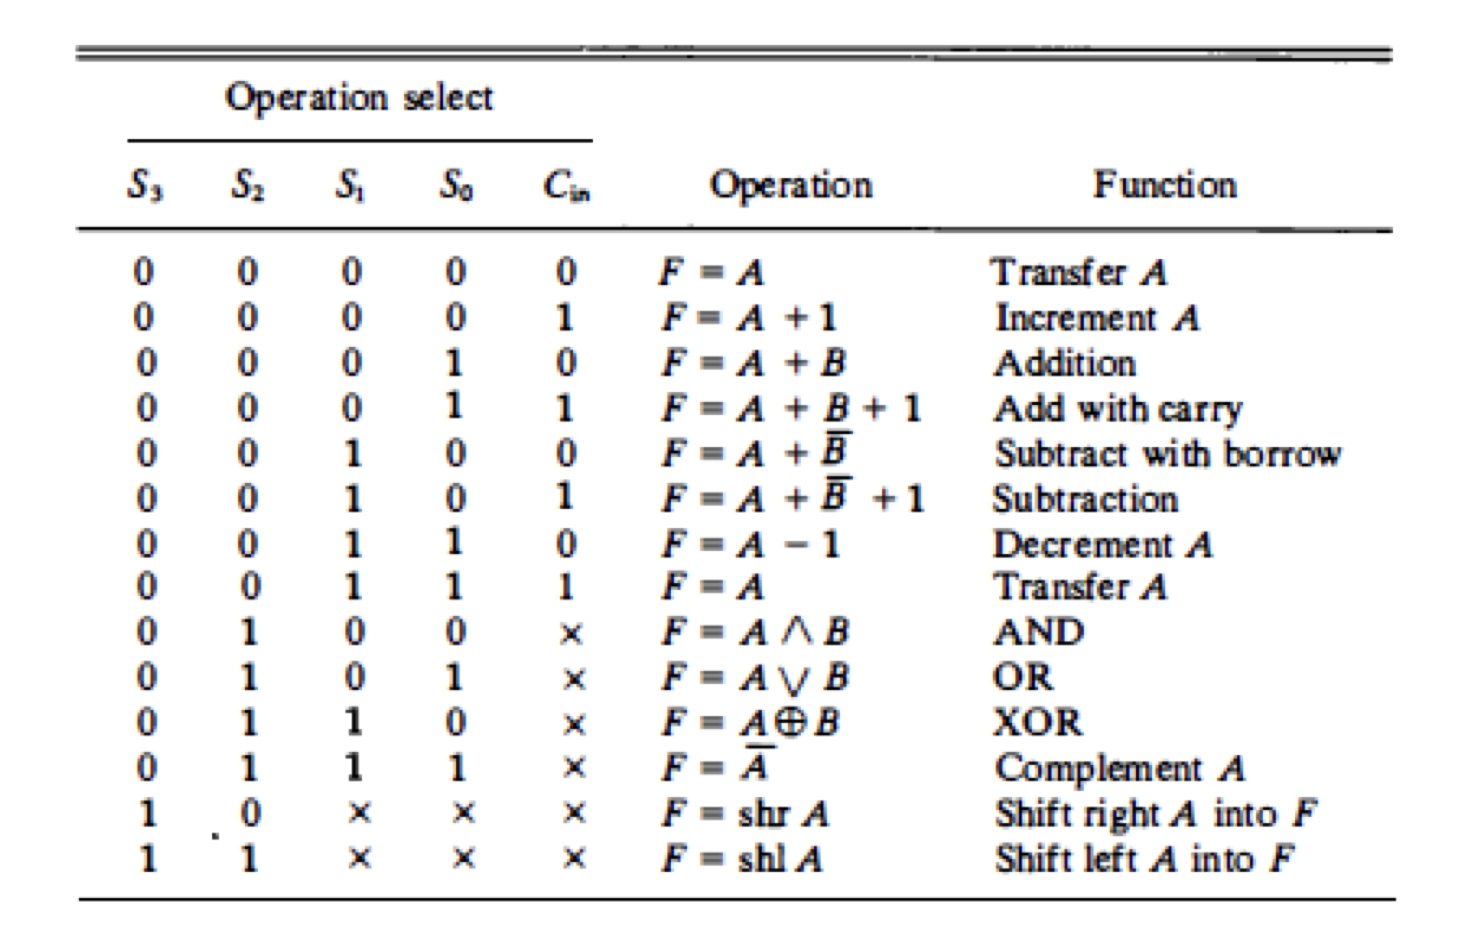
\includegraphics[width=\textwidth]{part2/table2.png}
    \caption{
    جدول عملکرد
    ALU
    که قرار است طراحی کنیم
    }
    \label{fig:table2}
\end{figure}

\subsection{بخش محاسبات Arithmetic}
بخش اول شامل ۸ دستور ابتدایی جدول است که به سادگی توسط یک تراشه‌ی جمع‌کننده پیاده‌سازی شده است.

مقدار کری به طور خودکار همیشه کافی است به ورودی کری جمع‌کننده اضافه شود و در همه‌ی بخش‌ها کار کند.

برای قسمت‌هایی که
B
قرار است مکمل ۱ شود باید همه‌ی بیت‌های آن را نات کنیم که این فرایند توسط گیت‌های
XOR
با یک ورودی مشترک
صورت می‌گیرد.

برای قسمت‌هایی که 
B
نباید حضور داشته باشد و 
،A
Decrement
می‌شود، کافی است
به جای B
چیزی که در جمع‌کننده با آن اضافه می‌شود، مکمل ۲ عدد منفی ۱ را اضافه کنیم که همان ۴ بیت ۱ است.

دو بیت کنترلی یکی مستقیم و دیگری با یک گیت به ورودی‌های ما مربوط می‌شوند که در شکل نهایی مدار آمده.

\subsection{بخش محاسبات Logical}
این بخش مستقیما توسط گیت‌ها پیاده‌سازی شده.
انتخاب بین خروجی گیت‌ها دوباره توسط دو
MUX
صورت می‌گیرد.

برای قسمت مکمل ۱ 
A
از روش مشابه قبل استفاده شده که در ورودی‌های
XOR
به جای
،B
۱
داده می‌شود تا بیت‌های
A
را قرینه کنند.

\subsection{بخش شیفت‌دهنده}
این بخش ساده‌ترین بخش است.
کافی است
A
را به صورت شیفت‌خورده به 
ورودی‌های
MUX
وصل کنیم.

در دو سری ورودی
MUX
هر بار یک بیت خالی می‌ماند که همان بیتی است که از ناکجا به داخل عدد شیفت‌خورده.
برای این بیت‌باید تصمیم بگیریم تراشه‌ی ما قرار است جه شیفتی انجام دهد.

یک راه این است که این ورودی را همان بیت کری ورودی قرار دهیم، یه می‌توانیم به سادگی آن را صفر قرار دهیم.
همچنین می‌توان آن را بیت علامت 
A
قرار داد.
در مدار فعلی این بیت‌ها صفر قرار داده‌شده‌اند اما به سادگی می‌توان آن را تغییر داد.

\begin{figure}[h!]
    \centering
    \includegraphics[width=\textwidth]{part2/ALU.png}
    \caption{
    مدار داخلی
    ALU
    }
\end{figure}